\documentclass[c5paper,twoside]{article} 
\usepackage{texthanglist}
\usepackage{multicol}
\usepackage{changepage}
\usepackage{float}
\usepackage{grffile}
\usepackage{graphicx}
\usepackage{amssymb}
\usepackage{fontspec}
\usepackage{fancyhdr}
\usepackage{multicol}
\usepackage{calc}
\usepackage[margin=1cm,includeheadfoot]{geometry}
\usepackage{eso-pic}
\pagestyle{plain}\pagestyle{fancy}
\fancyhead{}
\fancyhead[LO]{\rightmark}
\fancyhead[RO]{\thepage}
\fancyhead[LE]{\thepage}
\fancyhead[RE]{\leftmark}
\renewcommand{\headrulewidth}{0.4pt} \renewcommand{\footrulewidth}{0.4pt}
\fancyfoot{}

\begin{document} 
\pagestyle{plain} 
\font\spanenentryletDatadicBody="Times New Roman" at 10pt
\font\spantexitemtetranslationentranslationsexamplessensesensesentryletDatadicBody="Gautami" at 10pt
\font\xitemtetranslationentranslationsexamplessensesensesentryletDatadicBody="Gautami" at 10pt
\font\spanentranslationentranslationsexamplessensesensesentryletDatadicBody="Times New Roman" at 10pt
\font\spanenxitementranslationentranslationsexamplessensesensesentryletDatadicBody="Times New Roman" at 10pt
\font\xitementranslationentranslationsexamplessensesensesentryletDatadicBody="Times New Roman" at 10pt
\font\translationentranslationsexamplessensesensesentryletDatadicBody="Times New Roman" at 10pt
\font\spanenLexSensepublishStemGlossPubLehisensesensesentryletDatadicBody="Arial Unicode MS" at 10pt
\font\spanhiLexSensepublishStemGlossPubLehisensesensesentryletDatadicBody="Arial Unicode MS" at 10pt
\font\LexSensepublishStemGlossPubLehisensesensesentryletDatadicBody="Arial Unicode MS" at 10pt
\font\spanenpictureLabelenpictureCaptionpictureRightentryletDatadicBody="Times New Roman" at 10pt
\font\pictureLabelenpictureCaptionpictureRightentryletDatadicBody="Times New Roman" at 10pt
\font\spanenCmPicturepublishStemPileThumbnailPubpictureCaptionpictureRightentryletDatadicBody="Times New Roman" at 10pt
\font\CmPicturepublishStemPileThumbnailPubpictureCaptionpictureRightentryletDatadicBody="Times New Roman" at 10pt
\font\pictureCaptionpictureRightentryletDatadicBody="Times New Roman" at 10pt
\font\picturepictureRightentryletDatadicBody="Times New Roman" at 10pt
\font\pictureRightentryletDatadicBody="Times New Roman" at 10pt
\font\spanencomplexformrefsentryletDatadicBody="Times New Roman" at 10pt
\font\spanencomplexformformggoTeluINcomplexformrefsentryletDatadicBody="Gautami/B" at 10pt
\font\complexformformggoTeluINcomplexformrefsentryletDatadicBody="Gautami/B" at 10pt
\font\spanencomplexformtypecomplexformrefsentryletDatadicBody="Times New Roman" at 10pt
\font\spanenLexEntryTypepublishStemComplexFormTypeReverseAbbrPubencomplexformtypecomplexformrefsentryletDatadicBody="Times New Roman" at 10pt
\font\LexEntryTypepublishStemComplexFormTypeReverseAbbrPubencomplexformtypecomplexformrefsentryletDatadicBody="Times New Roman" at 10pt
\font\complexformtypecomplexformrefsentryletDatadicBody="Times New Roman" at 10pt
\font\complexformrefsentryletDatadicBody="Times New Roman" at 10pt
\font\spanentranslationLdtetranslationsexamplessensesensesentryletDatadicBody="Gautami" at 10pt
\font\spantetranslationLdtetranslationsexamplessensesensesentryletDatadicBody="Gautami" at 10pt
\font\translationLdtetranslationsexamplessensesensesentryletDatadicBody="Gautami" at 10pt
\font\translationsexamplessensesensesentryletDatadicBody="Times New Roman" at 10pt
\font\spanenexampleggoTeluINexamplessensesensesentryletDatadicBody="Gautami/I" at 10pt
\font\spanggoTeluINexampleggoTeluINexamplessensesensesentryletDatadicBody="Gautami/I" at 10pt
\font\exampleggoTeluINexamplessensesensesentryletDatadicBody="Gautami/I" at 10pt
\font\LexEntrypublishStemComponentTargetHeadWordRefggoTeluINaentryrefcomponentprimaryrefsentryletDatadicBody="Gautami/B" at 10pt
\font\aentryrefcomponentprimaryrefsentryletDatadicBody="Times New Roman" at 10pt
\font\entryrefcomponentprimaryrefsentryletDatadicBody="Times New Roman" at 10pt
\font\spanenentryreftypeprimaryrefsentryletDatadicBody="Times New Roman" at 10pt
\font\spanenLexEntryTypepublishStemEntryTypeAbbreviationPubenentryreftypeprimaryrefsentryletDatadicBody="Times New Roman" at 10pt
\font\LexEntryTypepublishStemEntryTypeAbbreviationPubenentryreftypeprimaryrefsentryletDatadicBody="Times New Roman" at 10pt
\font\entryreftypeprimaryrefsentryletDatadicBody="Times New Roman" at 10pt
\font\spanenprimaryrefsentryletDatadicBody="Times New Roman" at 10pt
\font\primaryrefsentryletDatadicBody="Times New Roman" at 10pt
\font\spanenexamplessensesensesentryletDatadicBody="Times New Roman" at 10pt
\font\spanentranslationLdtetranslationsxitemexamplessensesensesentryletDatadicBody="Gautami" at 10pt
\font\spantetranslationLdtetranslationsxitemexamplessensesensesentryletDatadicBody="Gautami" at 10pt
\font\translationLdtetranslationsxitemexamplessensesensesentryletDatadicBody="Gautami" at 10pt
\font\translationsxitemexamplessensesensesentryletDatadicBody="Times New Roman" at 10pt
\font\spanenexampleggoTeluINxitemexamplessensesensesentryletDatadicBody="Gautami/I" at 10pt
\font\spanggoTeluINexampleggoTeluINxitemexamplessensesensesentryletDatadicBody="Gautami/I" at 10pt
\font\exampleggoTeluINxitemexamplessensesensesentryletDatadicBody="Gautami/I" at 10pt
\font\xitemexamplessensesensesentryletDatadicBody="Times New Roman" at 10pt
\font\examplessensesensesentryletDatadicBody="Times New Roman" at 10pt
\font\spanhixitemhiLexSensepublishStemGlossPubLdtesensesensesentryletDatadicBody="Arial Unicode MS" at 10pt
\font\xitemhiLexSensepublishStemGlossPubLdtesensesensesentryletDatadicBody="Arial Unicode MS" at 10pt
\font\spantexitemteLexSensepublishStemGlossPubLdtesensesensesentryletDatadicBody="Gautami" at 10pt
\font\xitemteLexSensepublishStemGlossPubLdtesensesensesentryletDatadicBody="Gautami" at 10pt
\font\xsensenumberaftersensesensesentryletDatadicBody="Times New Roman" at 10pt
\font\xsensenumbersensesensesentryletDatadicBody="Times New Roman" at 10pt
\font\spanenpartofspeechengrammaticalinfoentryletDatadicBody="Times New Roman/I" at 10pt
\font\partofspeechengrammaticalinfoentryletDatadicBody="Times New Roman/I" at 10pt
\font\grammaticalinfoentryletDatadicBody="Times New Roman/I" at 10pt
\font\spanensensesentryletDatadicBody="Times New Roman" at 10pt
\font\spanenLexSensepublishStemGlossPubLdtesensesensesentryletDatadicBody="Gautami" at 10pt
\font\spanteLexSensepublishStemGlossPubLdtesensesensesentryletDatadicBody="Gautami" at 10pt
\font\LexSensepublishStemGlossPubLdtesensesensesentryletDatadicBody="Gautami" at 10pt
\font\spanendefinitionensensesensesentryletDatadicBody="Times New Roman" at 10pt
\font\definitionensensesensesentryletDatadicBody="Times New Roman" at 10pt
\font\spanengrammaticalinfosensesensesentryletDatadicBody="Times New Roman/I" at 10pt
\font\spanenpartofspeechengrammaticalinfosensesensesentryletDatadicBody="Times New Roman/I" at 10pt
\font\partofspeechengrammaticalinfosensesensesentryletDatadicBody="Times New Roman/I" at 10pt
\font\grammaticalinfosensesensesentryletDatadicBody="Times New Roman/I" at 10pt
\font\sensesensesentryletDatadicBody="Times New Roman" at 10pt
\font\sensesentryletDatadicBody="Times New Roman" at 10pt
\font\spanenpronunciationsentryletDatadicBody="Times New Roman" at 10pt
\font\spanggofonipaxemicpronunciationggofonipaxemicpronunciationsentryletDatadicBody="Tahoma" at 10pt
\font\spanenpronunciationggofonipaxemicpronunciationsentryletDatadicBody="Tahoma" at 10pt
\font\pronunciationggofonipaxemicpronunciationsentryletDatadicBody="Tahoma" at 10pt
\font\pronunciationsentryletDatadicBody="Times New Roman" at 10pt
\font\spanenheadwordggoTeluINentryletDatadicBody="Gautami/B" at 10pt
\font\headwordggoTeluINentryletDatadicBody="Gautami/B" at 10pt
\font\entryletDatadicBody="Times New Roman" at 10pt
\font\letDatadicBody="Times New Roman" at 12pt
\font\letterletHeaddicBody="Gautami/B" at 24pt
\font\letHeaddicBody="Times New Roman" at 12pt
\font\xitemtpi="Times New Roman" at 12pt
\font\xitemxitemtranslationLdbefore="Gautami" at 10pt
\font\xitemxitemtranslationbefore="Times New Roman" at 12pt
\font\sensesensesensesbefore="Times New Roman" at 12pt
\font\xitemxitempronunciationsbefore="Times New Roman" at 12pt
\font\xitemxitempronunciationbefore="Tahoma" at 10pt
\font\xitemxitemprimaryrefsbefore="Times New Roman" at 12pt
\font\xitemxitempictureLabelbefore="Times New Roman" at 12pt
\font\xitemxitempartofspeechbefore="Times New Roman" at 12pt
\font\xitemxitemLexSensepublishStemGlossPubLebefore="Arial Unicode MS" at 10pt
\font\xitemxitemLexSensepublishStemGlossPubLdbefore="Gautami" at 10pt
\font\xitemxitemLexEntryTypepublishStemEntryTypeAbbreviationPubbefore="Times New Roman" at 12pt
\font\xitemxitemLexEntryTypepublishStemComplexFormTypeReverseAbbrPubbefore="Times New Roman" at 12pt
\font\xitemxitemLexEntrypublishStemComponentTargetHeadWordRefbefore="Gautami/B" at 10pt
\font\xitemxitemheadwordbefore="Gautami/B" at 10pt
\font\xitemxitemexamplesbefore="Times New Roman" at 12pt
\font\xitemxitemexamplebefore="Gautami/I" at 10pt
\font\xitemxitementryreftypebefore="Times New Roman" at 12pt
\font\xitemxitementryrefcomponentbefore="Times New Roman" at 12pt
\font\xitemxitemdefinitionbefore="Times New Roman" at 12pt
\font\xitemxitemcomplexformrefsbefore="Times New Roman" at 12pt
\font\xitemxitemcomplexformformbefore="Gautami/B" at 10pt
\font\xitemhi="Arial Unicode MS" at 10pt
\font\xitemte="Gautami" at 10pt
\font\spanzhCN="SimSun" at 12pt
\font\divzhCN="SimSun" at 12pt
\font\spanvi="Charis SIL" at 12pt
\font\divvi="Charis SIL" at 12pt
\font\spantsi="Segoe UI" at 12pt
\font\divtsi="Segoe UI" at 12pt
\font\spantsiZxxxxaudio="Charis SIL" at 12pt
\font\divtsiZxxxxaudio="Charis SIL" at 12pt
\font\spantsixstr="Segoe UI" at 12pt
\font\divtsixstr="Segoe UI" at 12pt
\font\spantsifonipa="Segoe UI" at 12pt
\font\divtsifonipa="Segoe UI" at 12pt
\font\spantr="Charis SIL" at 12pt
\font\divtr="Charis SIL" at 12pt
\font\spantrfonipa="Doulos SIL" at 12pt
\font\divtrfonipa="Doulos SIL" at 12pt
\font\spantrfonipaxemic="Times New Roman" at 12pt
\font\divtrfonipaxemic="Times New Roman" at 12pt
\font\spantpi="Andika Basic" at 12pt
\font\divtpi="Andika Basic" at 12pt
\font\spanth="Angsana New" at 12pt
\font\divth="Angsana New" at 12pt
\font\spante="Gautami" at 12pt
\font\divte="Gautami" at 12pt
\font\spanswc="Times New Roman" at 12pt
\font\divswc="Times New Roman" at 12pt
\font\spanseh="Doulos SIL" at 12pt
\font\divseh="Doulos SIL" at 12pt
\font\spansehfonipaxetic="Doulos SIL" at 12pt
\font\divsehfonipaxetic="Doulos SIL" at 12pt
\font\spanru="Times New Roman" at 12pt
\font\divru="Times New Roman" at 12pt
\font\spanqaaxlel="Times New Roman" at 12pt
\font\divqaaxlel="Times New Roman" at 12pt
\font\spanpt="Times New Roman" at 12pt
\font\divpt="Times New Roman" at 12pt
\font\spannko="Charis SIL" at 12pt
\font\divnko="Charis SIL" at 12pt
\font\spanne="Mangal" at 12pt
\font\divne="Mangal" at 12pt
\font\spanmy="Padauk" at 12pt
\font\divmy="Padauk" at 12pt
\font\spanms="Charis SIL" at 12pt
\font\divms="Charis SIL" at 12pt
\font\spanlv="Times New Roman" at 12pt
\font\divlv="Times New Roman" at 12pt
\font\spankup="Charis SIL" at 12pt
\font\divkup="Charis SIL" at 12pt
\font\spanko="Gulim" at 12pt
\font\divko="Gulim" at 12pt
\font\spankm="DaunPenh" at 12pt
\font\divkm="DaunPenh" at 12pt
\font\spanid="Times New Roman" at 12pt
\font\divid="Times New Roman" at 12pt
\font\spanhi="Arial Unicode MS" at 12pt
\font\divhi="Arial Unicode MS" at 12pt
\font\spanhe="Ezra SIL" at 12pt
\font\divhe="Ezra SIL" at 12pt
\font\spanhbo="Ezra SIL" at 12pt
\font\divhbo="Ezra SIL" at 12pt
\font\spangrc="Galatia SIL" at 12pt
\font\divgrc="Galatia SIL" at 12pt
\font\spanggoTeluIN="Gautami" at 12pt
\font\divggoTeluIN="Gautami" at 12pt
\font\spanggofonipaxemic="Tahoma" at 12pt
\font\divggofonipaxemic="Tahoma" at 12pt
\font\spanfr="Times New Roman" at 12pt
\font\divfr="Times New Roman" at 12pt
\font\spanfrZxxxxaudio="Charis SIL" at 12pt
\font\divfrZxxxxaudio="Charis SIL" at 12pt
\font\spanflr="Doulos SIL" at 12pt
\font\divflr="Doulos SIL" at 12pt
\font\spanflrZxxxxaudio="Charis SIL" at 12pt
\font\divflrZxxxxaudio="Charis SIL" at 12pt
\font\spanflrQaaaxtone="Doulos SIL" at 12pt
\font\divflrQaaaxtone="Doulos SIL" at 12pt
\font\spanfa="Times New Roman" at 12pt
\font\divfa="Times New Roman" at 12pt
\font\spanes="Times New Roman" at 12pt
\font\dives="Times New Roman" at 12pt
\font\spanen="Times New Roman" at 12pt
\font\diven="Times New Roman" at 12pt
\font\spanenfonipa="Times New Roman" at 12pt
\font\divenfonipa="Times New Roman" at 12pt
\font\spande="Times New Roman" at 12pt
\font\divde="Times New Roman" at 12pt
\font\spanbzh="Charis SIL" at 12pt
\font\divbzh="Charis SIL" at 12pt
\font\spanbzhfonipa="Doulos SIL" at 12pt
\font\divbzhfonipa="Doulos SIL" at 12pt
\font\spanbn="Vrinda" at 12pt
\font\divbn="Vrinda" at 12pt
\font\spanbdu="Doulos SIL" at 12pt
\font\divbdu="Doulos SIL" at 12pt
\color{black} 
\AddToShipoutPicture*{% 
\put(0,0){\rule{\paperwidth}{\paperheight}}{
\includegraphics[width=\paperwidth, height=\paperheight]{cover.png}}% 
} 
\thispagestyle{empty} 
\font\CoverPageHeading="Times New Roman/B":color=000000 at 22pt 
\vskip 60pt 
\begin{center} 
\CoverPageHeading{Sample} 
\end{center} 
\newpage 
\newpage 
\thispagestyle{empty} 
\mbox{} 
\begin{titlepage}
\begin{center}
\textsc{\LARGE Sample}\\[1.5cm] 
\vspace{140 mm} 
\textsc{SIL International}\\[0.5cm] 
\includegraphics[width=0.05 \textwidth]{./SIL-Logo-No-Tag-Color.jpg}\\[1cm]    
\end{center} 
\end{titlepage} 
\newpage 
\newpage 
\mbox{} 
\pagenumbering{roman}  
\setcounter{page}{3} 
\input{SIL_CC-by-nc-sa.tex} 
\pagestyle{plain} 
\newpage 
\newpage 
\thispagestyle{empty} 
\mbox{} 

\addtocontents{toc}{\contentsline {section}{\numberline{} Words  అ - ొ}{\pageref{first_pageఅ}--\pageref{last_pageొ}}{}} 
\newpage 
\pagestyle{plain} 
\tableofcontents 
\newpage 
\setcounter{page}{1} 
\pagenumbering{arabic}  

\pagestyle{fancy} 
\begin{center}
\topskip 18pt{\baselineskip 18pt{\letterletHeaddicBody{అ}}}
 \label{first_pageఅ} \end{center}
 \setlength{\columnsep}{12pt} 
\setlength\columnseprule{0.4pt} 
\begin{multicols}{2}{\raggedright} \begin{adjustwidth}{1pt}{0pt}{2pt}{9pt}
 \begin{hanglist}[12pt] \item 
\leftmargin 0pt{\markboth{ \headwordggoTeluINentryletDatadicBody అకుర్పొక్ (మహ్న)}{ \headwordggoTeluINentryletDatadicBody అకుర్పొక్ (మహ్న)}\headwordggoTeluINentryletDatadicBody{అకుర్పొక్ (మహ్న)}} \spanenpronunciationggofonipaxemicpronunciationsentryletDatadicBody{[}\spanggofonipaxemicpronunciationggofonipaxemicpronunciationsentryletDatadicBody{akurpok (mahna)}\spanenpronunciationggofonipaxemicpronunciationsentryletDatadicBody{]} \spanenpartofspeechengrammaticalinfosensesensesentryletDatadicBody{n} \spanendefinitionensensesensesentryletDatadicBody{month 6 of the Gond year (August-September).} \spanteLexSensepublishStemGlossPubLdtesensesensesentryletDatadicBody{భాద్రపదం} \end{hanglist} \end{adjustwidth} 
\begin{adjustwidth}{1pt}{0pt}{2pt}{9pt}
 \begin{hanglist}[12pt] \item 
\leftmargin 0pt{\markboth{ \headwordggoTeluINentryletDatadicBody అకుర్పొక్ (మహ్న)}{ \headwordggoTeluINentryletDatadicBody అకుర్పొక్ (మహ్న)}\headwordggoTeluINentryletDatadicBody{అక్కల్}} \spanenpronunciationggofonipaxemicpronunciationsentryletDatadicBody{[}\spanggofonipaxemicpronunciationggofonipaxemicpronunciationsentryletDatadicBody{akkal}\spanenpronunciationggofonipaxemicpronunciationsentryletDatadicBody{]} \spanenpartofspeechengrammaticalinfoentryletDatadicBody{n} \xsensenumbersensesensesentryletDatadicBody{1}\xsensenumberaftersensesensesentryletDatadicBody{) }\spanteLexSensepublishStemGlossPubLdtesensesensesentryletDatadicBody{బుద్ధి} \xsensenumbersensesensesentryletDatadicBody{2}\xsensenumberaftersensesensesentryletDatadicBody{) }\spanendefinitionensensesensesentryletDatadicBody{wisdom.} \spantexitemteLexSensepublishStemGlossPubLdtesensesensesentryletDatadicBody{తెలివి} \spanhixitemhiLexSensepublishStemGlossPubLdtesensesensesentryletDatadicBody{बुद्धि} \spanggoTeluINexampleggoTeluINxitemexamplessensesensesentryletDatadicBody{అక్కల్ మన్వల్ మాయ్నల్ చొకొట్ మందంతొర్.} \spantetranslationLdtetranslationsxitemexamplessensesensesentryletDatadicBody{బుద్ధి గల వ్యక్తి మంచిగా ఉంటాడు.} \spanggoTeluINexampleggoTeluINxitemexamplessensesensesentryletDatadicBody{బయ్యె బాబలిర్ కాండిన్ అక్కల్ బుద్ది కరుసన.} \spantetranslationLdtetranslationsxitemexamplessensesensesentryletDatadicBody{తండ్రి తల్లి కొడుకులను తెలివి తేటలు నేర్పాలి.} \end{hanglist} \end{adjustwidth} 
\begin{adjustwidth}{1pt}{0pt}{2pt}{9pt}
 \begin{hanglist}[12pt] \item 
\leftmargin 0pt{\markboth{ \headwordggoTeluINentryletDatadicBody అక్కల్}{ \headwordggoTeluINentryletDatadicBody అక్కల్}\headwordggoTeluINentryletDatadicBody{అక్కొ మామల}} \spanenpronunciationggofonipaxemicpronunciationsentryletDatadicBody{[}\spanggofonipaxemicpronunciationggofonipaxemicpronunciationsentryletDatadicBody{akko māmal}\spanenpronunciationggofonipaxemicpronunciationsentryletDatadicBody{]} \spanenprimaryrefsentryletDatadicBody{(}\spanenLexEntryTypepublishStemEntryTypeAbbreviationPubenentryreftypeprimaryrefsentryletDatadicBody{der. of} \leftmargin 0pt{\LexEntrypublishStemComponentTargetHeadWordRefggoTeluINaentryrefcomponentprimaryrefsentryletDatadicBody{అక్కొ మామల్}}\spanenprimaryrefsentryletDatadicBody{) }\spanenpartofspeechengrammaticalinfosensesensesentryletDatadicBody{n} \spanteLexSensepublishStemGlossPubLdtesensesensesentryletDatadicBody{తాత మామయ్య} \spanggoTeluINexampleggoTeluINexamplessensesensesentryletDatadicBody{నన్ అక్కొ మామలిర్ సోరిక్ దాంతొన్.} \spantetranslationLdtetranslationsexamplessensesensesentryletDatadicBody{నేనూ తాతయ్య మామయ్య ఇంటికి సంబంధానికి వెలుతాను.} \end{hanglist} \end{adjustwidth} 
\begin{adjustwidth}{1pt}{0pt}{2pt}{9pt}
 \begin{hanglist}[12pt] \item 
\leftmargin 0pt{\markboth{ \headwordggoTeluINentryletDatadicBody అక్కొ మామల}{ \headwordggoTeluINentryletDatadicBody అక్కొ మామల}\headwordggoTeluINentryletDatadicBody{అక్కొ మామల్}} \spanenpronunciationggofonipaxemicpronunciationsentryletDatadicBody{[}\spanggofonipaxemicpronunciationggofonipaxemicpronunciationsentryletDatadicBody{akko}\spanenpronunciationggofonipaxemicpronunciationsentryletDatadicBody{]} \spanenpartofspeechengrammaticalinfosensesensesentryletDatadicBody{n} \spanendefinitionensensesensesentryletDatadicBody{maternal grandfather.} \spantexitemteLexSensepublishStemGlossPubLdtesensesensesentryletDatadicBody{తాత} \spanhixitemhiLexSensepublishStemGlossPubLdtesensesensesentryletDatadicBody{तात; नानादादा; बूढा आदमी} \spanggoTeluINexampleggoTeluINxitemexamplessensesensesentryletDatadicBody{మావొర్ అక్కొ డగుర్.} \spantetranslationLdtetranslationsxitemexamplessensesensesentryletDatadicBody{మా తాతయ్య పెద్దవాడు.} \spanggoTeluINexampleggoTeluINxitemexamplessensesensesentryletDatadicBody{అక్కొ చుట్ట ఉంజెర్ మంతొర్.} \spantetranslationLdtetranslationsxitemexamplessensesensesentryletDatadicBody{తాతయ్య చుట్ట తాగుతున్నాడు.} \spanenLexEntryTypepublishStemComplexFormTypeReverseAbbrPubencomplexformtypecomplexformrefsentryletDatadicBody{der.} \leftmargin 0pt{\complexformformggoTeluINcomplexformrefsentryletDatadicBody{అక్కొ మామల}} \end{hanglist} \end{adjustwidth} 
\begin{adjustwidth}{1pt}{0pt}{2pt}{9pt}
 \begin{hanglist}[12pt] \item 
\leftmargin 0pt{\markboth{ \headwordggoTeluINentryletDatadicBody అక్కొ మామల్}{ \headwordggoTeluINentryletDatadicBody అక్కొ మామల్}\headwordggoTeluINentryletDatadicBody{అక్డెమాత}} \spanenpronunciationggofonipaxemicpronunciationsentryletDatadicBody{[}\spanggofonipaxemicpronunciationggofonipaxemicpronunciationsentryletDatadicBody{akḍemāta}\spanenpronunciationggofonipaxemicpronunciationsentryletDatadicBody{]} \spanteLexSensepublishStemGlossPubLdtesensesensesentryletDatadicBody{ముడ్చుకున్నది} \spanggoTeluINexampleggoTeluINexamplessensesensesentryletDatadicBody{నావంగ్ కాల్క్ అక్డెమాతంగ్.} \spantetranslationLdtetranslationsexamplessensesensesentryletDatadicBody{నా కాళ్లు ముడ్చుకున్నాయి.} \end{hanglist} \end{adjustwidth} 
\begin{adjustwidth}{1pt}{0pt}{2pt}{9pt}
 \begin{hanglist}[12pt] \item 
\leftmargin 0pt{\markboth{ \headwordggoTeluINentryletDatadicBody అక్డెమాత}{ \headwordggoTeluINentryletDatadicBody అక్డెమాత}\headwordggoTeluINentryletDatadicBody{అక్ర}} \spanenpronunciationggofonipaxemicpronunciationsentryletDatadicBody{[}\spanggofonipaxemicpronunciationggofonipaxemicpronunciationsentryletDatadicBody{akra}\spanenpronunciationggofonipaxemicpronunciationsentryletDatadicBody{]} \spanenpartofspeechengrammaticalinfosensesensesentryletDatadicBody{num} \spanendefinitionensensesensesentryletDatadicBody{eleven.} \spantexitemteLexSensepublishStemGlossPubLdtesensesensesentryletDatadicBody{(11) పదకొండు} \spanhixitemhiLexSensepublishStemGlossPubLdtesensesensesentryletDatadicBody{ग्यारह} \spanggoTeluINexampleggoTeluINexamplessensesensesentryletDatadicBody{నాకున్ అక్ర హెర్రెంగ్ మంతంగ్.} \spantetranslationLdtetranslationsexamplessensesensesentryletDatadicBody{నాకు పదకొండు మేకలు ఉన్నాయి.} \end{hanglist} \end{adjustwidth} 
\begin{adjustwidth}{1pt}{0pt}{2pt}{9pt}
 \begin{hanglist}[12pt] \item 
\leftmargin 0pt{\markboth{ \headwordggoTeluINentryletDatadicBody అక్ర}{ \headwordggoTeluINentryletDatadicBody అక్ర}\headwordggoTeluINentryletDatadicBody{అక్సర్}} \spanenpronunciationggofonipaxemicpronunciationsentryletDatadicBody{[}\spanggofonipaxemicpronunciationggofonipaxemicpronunciationsentryletDatadicBody{aksar}\spanenpronunciationggofonipaxemicpronunciationsentryletDatadicBody{]} \spanenpartofspeechengrammaticalinfosensesensesentryletDatadicBody{n} \spanendefinitionensensesensesentryletDatadicBody{characters} \spanteLexSensepublishStemGlossPubLdtesensesensesentryletDatadicBody{అక్షరాలు} \spanggoTeluINexampleggoTeluINexamplessensesensesentryletDatadicBody{మస్తరల్ అక్సర్కున్ వెహ్తొర్.} \spantetranslationLdtetranslationsexamplessensesensesentryletDatadicBody{గురువు అక్షరాలు చెప్పాడు.} \end{hanglist} \end{adjustwidth} 
\begin{adjustwidth}{1pt}{0pt}{2pt}{9pt}
 \begin{hanglist}[12pt] \item 
\leftmargin 0pt{\markboth{ \headwordggoTeluINentryletDatadicBody అక్సర్}{ \headwordggoTeluINentryletDatadicBody అక్సర్}\headwordggoTeluINentryletDatadicBody{అక్సర్క్‌నె}} \spanenpronunciationggofonipaxemicpronunciationsentryletDatadicBody{[}\spanggofonipaxemicpronunciationggofonipaxemicpronunciationsentryletDatadicBody{aksarkne}\spanenpronunciationggofonipaxemicpronunciationsentryletDatadicBody{]} \spanteLexSensepublishStemGlossPubLdtesensesensesentryletDatadicBody{అచ్చరాలతో} \spanggoTeluINexampleggoTeluINexamplessensesensesentryletDatadicBody{గోండి బాసతున్ అక్సర్క్‌నె లిహి కీంతెర్.} \spantetranslationLdtetranslationsexamplessensesensesentryletDatadicBody{గోండిని అచ్చరాలలో రాసుకుంటారు.} \end{hanglist} \end{adjustwidth} 
\begin{adjustwidth}{1pt}{0pt}{2pt}{9pt}
 \begin{hanglist}[12pt] \item \begin{adjustwidth}{2pt}{2pt}{2pt}{2pt}\begin{center}

\begin{wrapfigure}
\begin{center}
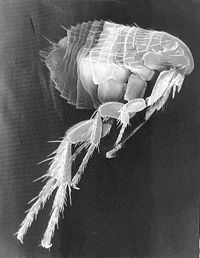
\includegraphics[angle=0,width=54mm,height=36mm]{1.jpg} 
\caption{}
\end{center}
\end{wrapfigure}



\spanenpictureLabelenpictureCaptionpictureRightentryletDatadicBody{rice with tumeric}
\end{center}\end{adjustwidth}  
\leftmargin 0pt{\markboth{ \headwordggoTeluINentryletDatadicBody అక్సర్క్‌నె}{ \headwordggoTeluINentryletDatadicBody అక్సర్క్‌నె}\headwordggoTeluINentryletDatadicBody{అక్సెదంగ్}} \spanenpronunciationggofonipaxemicpronunciationsentryletDatadicBody{[}\spanggofonipaxemicpronunciationggofonipaxemicpronunciationsentryletDatadicBody{aksedaṅg}\spanenpronunciationggofonipaxemicpronunciationsentryletDatadicBody{]} \spanenpartofspeechengrammaticalinfoentryletDatadicBody{n} \xsensenumbersensesensesentryletDatadicBody{1}\xsensenumberaftersensesensesentryletDatadicBody{) }\spanendefinitionensensesensesentryletDatadicBody{rice with vermilion} \spanteLexSensepublishStemGlossPubLdtesensesensesentryletDatadicBody{పసుపు బియ్యం} \xsensenumbersensesensesentryletDatadicBody{2}\xsensenumberaftersensesensesentryletDatadicBody{) }\spanendefinitionensensesensesentryletDatadicBody{rice mixed with vermilion thrown at a wedding, or on cattle (e.g. during 'laxmi pooja') in order to bless.} \spanhiLexSensepublishStemGlossPubLehisensesensesentryletDatadicBody{अक्षतब.; हल्दी और कुंकुम से मिश्रित चावल} \spanggoTeluINexampleggoTeluINexamplessensesensesentryletDatadicBody{గొవుర్ దన్ గోటమ్నె నొవ్రి నొవ్రనగ సమ్దిర్ అక్సెదాంగ్ వాటంతెర్.} \spanenxitementranslationentranslationsexamplessensesensesentryletDatadicBody{At the wedding place, everyone throws rice on the bride andgroom.} \spantexitemtetranslationentranslationsexamplessensesensesentryletDatadicBody{$\sharp$పెండ్లి పందిరిలో పడుసు, వరులకు పసుపు బియ్యం వేస్తారు.} \end{hanglist} \end{adjustwidth} 
\begin{adjustwidth}{1pt}{0pt}{2pt}{9pt}
 \begin{hanglist}[12pt] \item 
\leftmargin 0pt{\markboth{ \headwordggoTeluINentryletDatadicBody అక్సెదంగ్}{ \headwordggoTeluINentryletDatadicBody అక్సెదంగ్}\headwordggoTeluINentryletDatadicBody{అక్సెదన దివొస్}} \spanenpronunciationggofonipaxemicpronunciationsentryletDatadicBody{[}\spanggofonipaxemicpronunciationggofonipaxemicpronunciationsentryletDatadicBody{aksedana divos}\spanenpronunciationggofonipaxemicpronunciationsentryletDatadicBody{]} \spanendefinitionensensesensesentryletDatadicBody{wedding day} \spanteLexSensepublishStemGlossPubLdtesensesensesentryletDatadicBody{పెళ్లి రోజు} \end{hanglist} \end{adjustwidth} 
\begin{adjustwidth}{1pt}{0pt}{2pt}{9pt}
 \begin{hanglist}[12pt] \item 
\leftmargin 0pt{\markboth{ \headwordggoTeluINentryletDatadicBody అక్సెదన దివొస్}{ \headwordggoTeluINentryletDatadicBody అక్సెదన దివొస్}\headwordggoTeluINentryletDatadicBody{అక్సెర్}} \spanenpronunciationggofonipaxemicpronunciationsentryletDatadicBody{[}\spanggofonipaxemicpronunciationggofonipaxemicpronunciationsentryletDatadicBody{akser}\spanenpronunciationggofonipaxemicpronunciationsentryletDatadicBody{]} \spanenpartofspeechengrammaticalinfosensesensesentryletDatadicBody{n} \spanendefinitionensensesensesentryletDatadicBody{character} \spantexitemteLexSensepublishStemGlossPubLdtesensesensesentryletDatadicBody{అక్షరం} \spanhixitemhiLexSensepublishStemGlossPubLdtesensesensesentryletDatadicBody{अक्षर; वर्ण} \spanggoTeluINexampleggoTeluINexamplessensesensesentryletDatadicBody{అక్సెర్ ఉంది గునం.} \spantetranslationLdtetranslationsexamplessensesensesentryletDatadicBody{అక్షరం ఉంది గుణం.} \end{hanglist} \end{adjustwidth} 
\begin{adjustwidth}{1pt}{0pt}{2pt}{9pt}
 \begin{hanglist}[12pt] \item 
\leftmargin 0pt{\markboth{ \headwordggoTeluINentryletDatadicBody అక్సెర్}{ \headwordggoTeluINentryletDatadicBody అక్సెర్}\headwordggoTeluINentryletDatadicBody{అగ్గటల్}} \spanenpronunciationggofonipaxemicpronunciationsentryletDatadicBody{[}\spanggofonipaxemicpronunciationggofonipaxemicpronunciationsentryletDatadicBody{aggaṭal}\spanenpronunciationggofonipaxemicpronunciationsentryletDatadicBody{]} \spanenpartofspeechengrammaticalinfoentryletDatadicBody{adv} \xsensenumbersensesensesentryletDatadicBody{1}\xsensenumberaftersensesensesentryletDatadicBody{) }\spanendefinitionensensesensesentryletDatadicBody{from there (nm.)} \spantexitemteLexSensepublishStemGlossPubLdtesensesensesentryletDatadicBody{నుంచి} \spanhixitemhiLexSensepublishStemGlossPubLdtesensesensesentryletDatadicBody{वहा से} \xsensenumbersensesensesentryletDatadicBody{2}\xsensenumberaftersensesensesentryletDatadicBody{) }\spanendefinitionensensesensesentryletDatadicBody{someone (nm.) or something from there.} \spanteLexSensepublishStemGlossPubLdtesensesensesentryletDatadicBody{అక్కడనుండి} \spanggoTeluINexampleggoTeluINexamplessensesensesentryletDatadicBody{అగ్గటల్ నన్న నీకున్ సూడ్తొన్.} \spantetranslationLdtetranslationsexamplessensesensesentryletDatadicBody{అక్కడి నుండి నేను నిన్ను చూసాను.} \end{hanglist} \end{adjustwidth} 
\begin{adjustwidth}{1pt}{0pt}{2pt}{9pt}
 \begin{hanglist}[12pt] \item 
\leftmargin 0pt{\markboth{ \headwordggoTeluINentryletDatadicBody అగ్గటల్}{ \headwordggoTeluINentryletDatadicBody అగ్గటల్}\headwordggoTeluINentryletDatadicBody{అగ్గటొర}} \spanenpronunciationggofonipaxemicpronunciationsentryletDatadicBody{[}\spanggofonipaxemicpronunciationggofonipaxemicpronunciationsentryletDatadicBody{aggaṭor}\spanenpronunciationggofonipaxemicpronunciationsentryletDatadicBody{]} \spanenprimaryrefsentryletDatadicBody{(}\spanenLexEntryTypepublishStemEntryTypeAbbreviationPubenentryreftypeprimaryrefsentryletDatadicBody{der. of} \leftmargin 0pt{\LexEntrypublishStemComponentTargetHeadWordRefggoTeluINaentryrefcomponentprimaryrefsentryletDatadicBody{అగ్గటొర్}}\spanenprimaryrefsentryletDatadicBody{) }\spanenpartofspeechengrammaticalinfosensesensesentryletDatadicBody{n} \spanendefinitionensensesensesentryletDatadicBody{man from there.} \spanteLexSensepublishStemGlossPubLdtesensesensesentryletDatadicBody{అక్కడివారు} \spanggoTeluINexampleggoTeluINexamplessensesensesentryletDatadicBody{వేర్ మాయ్నల్ అగ్గటొర్.} \spanenxitementranslationentranslationsexamplessensesensesentryletDatadicBody{This man is from there.} \spantexitemtetranslationentranslationsexamplessensesensesentryletDatadicBody{ఈ వ్యక్తి అక్కడి వారు.} \end{hanglist} \end{adjustwidth} 
\begin{adjustwidth}{1pt}{0pt}{2pt}{9pt}
 \begin{hanglist}[12pt] \item 
\leftmargin 0pt{\markboth{ \headwordggoTeluINentryletDatadicBody అగ్గటొర}{ \headwordggoTeluINentryletDatadicBody అగ్గటొర}\headwordggoTeluINentryletDatadicBody{అగ్గటొర్}} \spanenpronunciationggofonipaxemicpronunciationsentryletDatadicBody{[}\spanggofonipaxemicpronunciationggofonipaxemicpronunciationsentryletDatadicBody{agga}\spanenpronunciationggofonipaxemicpronunciationsentryletDatadicBody{]} \xsensenumbersensesensesentryletDatadicBody{1}\xsensenumberaftersensesensesentryletDatadicBody{) }\spanenpartofspeechengrammaticalinfosensesensesentryletDatadicBody{adv} \spanendefinitionensensesensesentryletDatadicBody{there.} \spantexitemteLexSensepublishStemGlossPubLdtesensesensesentryletDatadicBody{అక్కడ} \spanhixitemhiLexSensepublishStemGlossPubLdtesensesensesentryletDatadicBody{वहा} \spanggoTeluINexampleggoTeluINexamplessensesensesentryletDatadicBody{వేర్ వెర్తల్ అగ్గటొర్ ఆందుర్.} \spantetranslationLdtetranslationsexamplessensesensesentryletDatadicBody{ఈ చుట్టము అక్కడి వాడు.} \xsensenumbersensesensesentryletDatadicBody{2}\xsensenumberaftersensesensesentryletDatadicBody{) }\spanendefinitionensensesensesentryletDatadicBody{there} \spanenLexEntryTypepublishStemComplexFormTypeReverseAbbrPubencomplexformtypecomplexformrefsentryletDatadicBody{der.} \leftmargin 0pt{\complexformformggoTeluINcomplexformrefsentryletDatadicBody{అగ్గటొర}} \end{hanglist} \end{adjustwidth} 
\begin{adjustwidth}{1pt}{0pt}{2pt}{9pt}
 \begin{hanglist}[12pt] \item 
\leftmargin 0pt{\markboth{ \headwordggoTeluINentryletDatadicBody అగ్గటొర్}{ \headwordggoTeluINentryletDatadicBody అగ్గటొర్}\headwordggoTeluINentryletDatadicBody{అఙె}} \spanenpronunciationggofonipaxemicpronunciationsentryletDatadicBody{[}\spanggofonipaxemicpronunciationggofonipaxemicpronunciationsentryletDatadicBody{aṅe}\spanenpronunciationggofonipaxemicpronunciationsentryletDatadicBody{]} \spanenpartofspeechengrammaticalinfosensesensesentryletDatadicBody{n} \spanendefinitionensensesensesentryletDatadicBody{elder brother's wife.} \spantexitemteLexSensepublishStemGlossPubLdtesensesensesentryletDatadicBody{వదిన} \spanhixitemhiLexSensepublishStemGlossPubLdtesensesensesentryletDatadicBody{भाबि} \spanggoTeluINexampleggoTeluINexamplessensesensesentryletDatadicBody{మావొర్ దాదన బాయ్కొ నాకున్ అఙె ఆంత.} \spantetranslationLdtetranslationsexamplessensesensesentryletDatadicBody{మా అన్నయ్య పెండ్లం నాకు వదిన అవుతుంది.} \end{hanglist} \end{adjustwidth} 
\begin{adjustwidth}{1pt}{0pt}{2pt}{9pt}
 \begin{hanglist}[12pt] \item 
\leftmargin 0pt{\markboth{ \headwordggoTeluINentryletDatadicBody అఙె}{ \headwordggoTeluINentryletDatadicBody అఙె}\headwordggoTeluINentryletDatadicBody{అచనక్}} \spanenpronunciationggofonipaxemicpronunciationsentryletDatadicBody{[}\spanggofonipaxemicpronunciationggofonipaxemicpronunciationsentryletDatadicBody{acanak}\spanenpronunciationggofonipaxemicpronunciationsentryletDatadicBody{]} \spanenpartofspeechengrammaticalinfosensesensesentryletDatadicBody{adv} \spanendefinitionensensesensesentryletDatadicBody{suddenly} \spanteLexSensepublishStemGlossPubLdtesensesensesentryletDatadicBody{ఆకస్మికంగా} \spanggoTeluINexampleggoTeluINexamplessensesensesentryletDatadicBody{మావ సాడతె అచనక్ పి.ఓ. సాబ్ వాసి మత్తొర్.} \spantetranslationLdtetranslationsexamplessensesensesentryletDatadicBody{మా బడికి పి.ఓ ఆకస్మికంగా వచ్చినాడు.} \end{hanglist} \end{adjustwidth} 
\begin{adjustwidth}{1pt}{0pt}{2pt}{9pt}
 \begin{hanglist}[12pt] \item 
\leftmargin 0pt{\markboth{ \headwordggoTeluINentryletDatadicBody అచనక్}{ \headwordggoTeluINentryletDatadicBody అచనక్}\headwordggoTeluINentryletDatadicBody{అచొట్క్}} \spanenpronunciationggofonipaxemicpronunciationsentryletDatadicBody{[}\spanggofonipaxemicpronunciationggofonipaxemicpronunciationsentryletDatadicBody{acoṭk}\spanenpronunciationggofonipaxemicpronunciationsentryletDatadicBody{]} \spanenpartofspeechengrammaticalinfosensesensesentryletDatadicBody{n} \spanendefinitionensensesensesentryletDatadicBody{usual} \spantexitemteLexSensepublishStemGlossPubLdtesensesensesentryletDatadicBody{మామూలు} \spanhixitemhiLexSensepublishStemGlossPubLdtesensesensesentryletDatadicBody{साधारण} \end{hanglist} \end{adjustwidth} 
\begin{adjustwidth}{1pt}{0pt}{2pt}{9pt}
 \begin{hanglist}[12pt] \item 
\leftmargin 0pt{\markboth{ \headwordggoTeluINentryletDatadicBody అచొట్క్}{ \headwordggoTeluINentryletDatadicBody అచొట్క్}\headwordggoTeluINentryletDatadicBody{అచ్చొరె}} \spanenpronunciationggofonipaxemicpronunciationsentryletDatadicBody{[}\spanggofonipaxemicpronunciationggofonipaxemicpronunciationsentryletDatadicBody{accore}\spanenpronunciationggofonipaxemicpronunciationsentryletDatadicBody{]} \xsensenumbersensesensesentryletDatadicBody{1}\xsensenumberaftersensesensesentryletDatadicBody{) }\spanteLexSensepublishStemGlossPubLdtesensesensesentryletDatadicBody{ఇంతే} \spanggoTeluINexampleggoTeluINexamplessensesensesentryletDatadicBody{కాండిరంగ్ పరిక్సంగ్ అచ్చొరె.} \spantetranslationLdtetranslationsexamplessensesensesentryletDatadicBody{పిల్లల పరీక్షలు ఇంతే.} \xsensenumbersensesensesentryletDatadicBody{2}\xsensenumberaftersensesensesentryletDatadicBody{) }\spanendefinitionensensesensesentryletDatadicBody{that's all} \end{hanglist} \end{adjustwidth} 
\begin{adjustwidth}{1pt}{0pt}{2pt}{9pt}
 \begin{hanglist}[12pt] \item 
\leftmargin 0pt{\markboth{ \headwordggoTeluINentryletDatadicBody అచ్చొరె}{ \headwordggoTeluINentryletDatadicBody అచ్చొరె}\headwordggoTeluINentryletDatadicBody{అచ్చొర్}} \spanenpronunciationggofonipaxemicpronunciationsentryletDatadicBody{[}\spanggofonipaxemicpronunciationggofonipaxemicpronunciationsentryletDatadicBody{accor}\spanenpronunciationggofonipaxemicpronunciationsentryletDatadicBody{]} \spanenpartofspeechengrammaticalinfosensesensesentryletDatadicBody{adv} \spanendefinitionensensesensesentryletDatadicBody{that much, that many (nm.).} \spanteLexSensepublishStemGlossPubLdtesensesensesentryletDatadicBody{అంత} \spanggoTeluINexampleggoTeluINexamplessensesensesentryletDatadicBody{నిమ్మె అచ్చొర్ డగుర్ బహన్ ఆతి.} \spantetranslationLdtetranslationsexamplessensesensesentryletDatadicBody{నీవు అంత పెద్దగా ఏలా అయినావు.} \spanenLexEntryTypepublishStemComplexFormTypeReverseAbbrPubencomplexformtypecomplexformrefsentryletDatadicBody{der.} \leftmargin 0pt{\complexformformggoTeluINcomplexformrefsentryletDatadicBody{అచ్చోడ్ రొప్పొ}} \end{hanglist} \end{adjustwidth} 
\begin{adjustwidth}{1pt}{0pt}{2pt}{9pt}
 \begin{hanglist}[12pt] \item 
\leftmargin 0pt{\markboth{ \headwordggoTeluINentryletDatadicBody అచ్చొర్}{ \headwordggoTeluINentryletDatadicBody అచ్చొర్}\headwordggoTeluINentryletDatadicBody{అచ్చోడ్ రొప్పొ}} \spanenpronunciationggofonipaxemicpronunciationsentryletDatadicBody{[}\spanggofonipaxemicpronunciationggofonipaxemicpronunciationsentryletDatadicBody{accōḍ roppo}\spanenpronunciationggofonipaxemicpronunciationsentryletDatadicBody{]} \spanenprimaryrefsentryletDatadicBody{(}\spanenLexEntryTypepublishStemEntryTypeAbbreviationPubenentryreftypeprimaryrefsentryletDatadicBody{der. of} \leftmargin 0pt{\LexEntrypublishStemComponentTargetHeadWordRefggoTeluINaentryrefcomponentprimaryrefsentryletDatadicBody{అచ్చొర్}}\spanenprimaryrefsentryletDatadicBody{) }\spanenpartofspeechengrammaticalinfosensesensesentryletDatadicBody{adv} \spanendefinitionensensesensesentryletDatadicBody{meanwhile.} \spantexitemteLexSensepublishStemGlossPubLdtesensesensesentryletDatadicBody{అంతలో} \spanhixitemhiLexSensepublishStemGlossPubLdtesensesensesentryletDatadicBody{इसी दौरान} \spanggoTeluINexampleggoTeluINexamplessensesensesentryletDatadicBody{బుయరితగ అచ్చొడ్ రొప్పొ నేంగ్మా.} \spantetranslationLdtetranslationsexamplessensesensesentryletDatadicBody{గుహలో చాల లోపలికి వెళ్లకు.} \end{hanglist} \end{adjustwidth} 
\begin{adjustwidth}{1pt}{0pt}{2pt}{9pt}
 \begin{hanglist}[12pt] \item 
\leftmargin 0pt{\markboth{ \headwordggoTeluINentryletDatadicBody అచ్చోడ్ రొప్పొ}{ \headwordggoTeluINentryletDatadicBody అచ్చోడ్ రొప్పొ}\headwordggoTeluINentryletDatadicBody{అచ్వీర్}} \spanenpronunciationggofonipaxemicpronunciationsentryletDatadicBody{[}\spanggofonipaxemicpronunciationggofonipaxemicpronunciationsentryletDatadicBody{acvīr}\spanenpronunciationggofonipaxemicpronunciationsentryletDatadicBody{]} \spanenpartofspeechengrammaticalinfosensesensesentryletDatadicBody{pro} \spanendefinitionensensesensesentryletDatadicBody{that many (m.).} \spanteLexSensepublishStemGlossPubLdtesensesensesentryletDatadicBody{అంతమంది} \spanggoTeluINexampleggoTeluINexamplessensesensesentryletDatadicBody{అచ్విర్ తె మావ రోన్ తిన్లెన్ వాయన.} \spantetranslationLdtetranslationsexamplessensesensesentryletDatadicBody{అంతమంది మా ఇంటికి తినడానికి రావాలి.} \end{hanglist} \end{adjustwidth} 
\begin{adjustwidth}{1pt}{0pt}{2pt}{9pt}
 \begin{hanglist}[12pt] \item 
\leftmargin 0pt{\markboth{ \headwordggoTeluINentryletDatadicBody అచ్వీర్}{ \headwordggoTeluINentryletDatadicBody అచ్వీర్}\headwordggoTeluINentryletDatadicBody{అజుక్}} \spanenpronunciationggofonipaxemicpronunciationsentryletDatadicBody{[}\spanggofonipaxemicpronunciationggofonipaxemicpronunciationsentryletDatadicBody{ajuk}\spanenpronunciationggofonipaxemicpronunciationsentryletDatadicBody{]} \spanenpartofspeechengrammaticalinfosensesensesentryletDatadicBody{conj} \spanendefinitionensensesensesentryletDatadicBody{even now.} \spanteLexSensepublishStemGlossPubLdtesensesensesentryletDatadicBody{ఇంకా} \spanggoTeluINexampleggoTeluINexamplessensesensesentryletDatadicBody{దుకాన్ దారల్ అజుక్ ఉండె బతంగ్ పహజ్లె ఇంతొర్.} \spantetranslationLdtetranslationsexamplessensesensesentryletDatadicBody{దుకాణ దారు ఇంకా ఏమి కావాలి అని అడుగుతున్నాడు.} \end{hanglist} \end{adjustwidth} 
\begin{adjustwidth}{1pt}{0pt}{2pt}{9pt}
 \begin{hanglist}[12pt] \item 
\leftmargin 0pt{\markboth{ \headwordggoTeluINentryletDatadicBody అజుక్}{ \headwordggoTeluINentryletDatadicBody అజుక్}\headwordggoTeluINentryletDatadicBody{అటుమ్ కుటుమ్}} \spanenpronunciationggofonipaxemicpronunciationsentryletDatadicBody{[}\spanggofonipaxemicpronunciationggofonipaxemicpronunciationsentryletDatadicBody{aṭum kuṭum}\spanenpronunciationggofonipaxemicpronunciationsentryletDatadicBody{]} \spanteLexSensepublishStemGlossPubLdtesensesensesentryletDatadicBody{చుట్టలు చుట్టం} \spanggoTeluINexampleggoTeluINexamplessensesensesentryletDatadicBody{మర్మిన్క్ అటుమ్ కుటుమున్ సమ్దిర్క్ కేయంతెర్.} \spantetranslationLdtetranslationsexamplessensesensesentryletDatadicBody{పెండ్లిలో చుట్టలు చుట్టాలు అందరిని పిలుస్తారు.} \end{hanglist} \end{adjustwidth} 
\begin{adjustwidth}{1pt}{0pt}{2pt}{9pt}
 \begin{hanglist}[12pt] \item 
\leftmargin 0pt{\markboth{ \headwordggoTeluINentryletDatadicBody అటుమ్ కుటుమ్}{ \headwordggoTeluINentryletDatadicBody అటుమ్ కుటుమ్}\headwordggoTeluINentryletDatadicBody{అటొ}} \spanenpronunciationggofonipaxemicpronunciationsentryletDatadicBody{[}\spanggofonipaxemicpronunciationggofonipaxemicpronunciationsentryletDatadicBody{aṭo}\spanenpronunciationggofonipaxemicpronunciationsentryletDatadicBody{]} \spanenpartofspeechengrammaticalinfosensesensesentryletDatadicBody{n} \spanendefinitionensensesensesentryletDatadicBody{auto} \spanteLexSensepublishStemGlossPubLdtesensesensesentryletDatadicBody{ఆటో} \spanggoTeluINexampleggoTeluINexamplessensesensesentryletDatadicBody{అటొతున్ మూంద్ గారెంగ్ మందంతంగ్.} \spantetranslationLdtetranslationsexamplessensesensesentryletDatadicBody{ఆటో కు మూడు చక్రాలు ఉంటాయి.} \end{hanglist} \end{adjustwidth} 
\begin{adjustwidth}{1pt}{0pt}{2pt}{9pt}
 \begin{hanglist}[12pt] \item 
\leftmargin 0pt{\markboth{ \headwordggoTeluINentryletDatadicBody అటొ}{ \headwordggoTeluINentryletDatadicBody అటొ}\headwordggoTeluINentryletDatadicBody{అట్కీ కీత}} \spanenpronunciationggofonipaxemicpronunciationsentryletDatadicBody{[}\spanggofonipaxemicpronunciationggofonipaxemicpronunciationsentryletDatadicBody{aṭki kī-}\spanenpronunciationggofonipaxemicpronunciationsentryletDatadicBody{]} \spanenpartofspeechengrammaticalinfoentryletDatadicBody{n} \xsensenumbersensesensesentryletDatadicBody{1}\xsensenumberaftersensesensesentryletDatadicBody{) }\spanendefinitionensensesensesentryletDatadicBody{fixation} \spanteLexSensepublishStemGlossPubLdtesensesensesentryletDatadicBody{అంటించడం} \xsensenumbersensesensesentryletDatadicBody{2}\xsensenumberaftersensesensesentryletDatadicBody{) }\spanendefinitionensensesensesentryletDatadicBody{to hang.} \spanhiLexSensepublishStemGlossPubLehisensesensesentryletDatadicBody{टाँगना} \spanggoTeluINexampleggoTeluINexamplessensesensesentryletDatadicBody{నావ ఆంగ్డెతున్ మోలతగ అట్కి కీతొన్.} \spantetranslationLdtetranslationsexamplessensesensesentryletDatadicBody{నా అంగిని మొలలో అంటి పెట్టుకున్నాను.} \end{hanglist} \end{adjustwidth} 
\begin{adjustwidth}{1pt}{0pt}{2pt}{9pt}
 \begin{hanglist}[12pt] \item 
\leftmargin 0pt{\markboth{ \headwordggoTeluINentryletDatadicBody అట్కీ కీత}{ \headwordggoTeluINentryletDatadicBody అట్కీ కీత}\headwordggoTeluINentryletDatadicBody{అట్కుల్క్}} \spanenpronunciationggofonipaxemicpronunciationsentryletDatadicBody{[}\spanggofonipaxemicpronunciationggofonipaxemicpronunciationsentryletDatadicBody{aṭkulk}\spanenpronunciationggofonipaxemicpronunciationsentryletDatadicBody{]} \spanenpartofspeechengrammaticalinfosensesensesentryletDatadicBody{n} \spanendefinitionensensesensesentryletDatadicBody{flattened rice} \spantexitemteLexSensepublishStemGlossPubLdtesensesensesentryletDatadicBody{అటుకులు} \spanhixitemhiLexSensepublishStemGlossPubLdtesensesensesentryletDatadicBody{चिउडा} \spanggoTeluINexampleggoTeluINexamplessensesensesentryletDatadicBody{పెరెక్ ఙల్ అట్కుల్క్ తయర్ కీంతెర్.} \spantetranslationLdtetranslationsexamplessensesensesentryletDatadicBody{బియ్యము నుండి అటుకులు తయారు చేస్తారు.} \end{hanglist} \end{adjustwidth} 
\begin{adjustwidth}{1pt}{0pt}{2pt}{9pt}
 \begin{hanglist}[12pt] \item 
\leftmargin 0pt{\markboth{ \headwordggoTeluINentryletDatadicBody అట్కుల్క్}{ \headwordggoTeluINentryletDatadicBody అట్కుల్క్}\headwordggoTeluINentryletDatadicBody{అట్కె మాత}} \spanenpronunciationggofonipaxemicpronunciationsentryletDatadicBody{[}\spanggofonipaxemicpronunciationggofonipaxemicpronunciationsentryletDatadicBody{aṭke māta}\spanenpronunciationggofonipaxemicpronunciationsentryletDatadicBody{]} \spanteLexSensepublishStemGlossPubLdtesensesensesentryletDatadicBody{ఊపిరి ఆగింది} \spanggoTeluINexampleggoTeluINexamplessensesensesentryletDatadicBody{నావ నేస్క్‌వల్ అట్కె మాత.} \spantetranslationLdtetranslationsexamplessensesensesentryletDatadicBody{నా ఊపిరి ఆగిపోయింది.} \end{hanglist} \end{adjustwidth} 
\begin{adjustwidth}{1pt}{0pt}{2pt}{9pt}
 \begin{hanglist}[12pt] \item 
\leftmargin 0pt{\markboth{ \headwordggoTeluINentryletDatadicBody అట్కె మాత}{ \headwordggoTeluINentryletDatadicBody అట్కె మాత}\headwordggoTeluINentryletDatadicBody{అట్ట}} \spanenpronunciationggofonipaxemicpronunciationsentryletDatadicBody{[}\spanggofonipaxemicpronunciationggofonipaxemicpronunciationsentryletDatadicBody{aṭṭa}\spanenpronunciationggofonipaxemicpronunciationsentryletDatadicBody{]} \spanendefinitionensensesensesentryletDatadicBody{cook} \spanteLexSensepublishStemGlossPubLdtesensesensesentryletDatadicBody{వంట చెయ్యి} \end{hanglist} \end{adjustwidth} 
\begin{adjustwidth}{1pt}{0pt}{2pt}{9pt}
 \begin{hanglist}[12pt] \item 
\leftmargin 0pt{\markboth{ \headwordggoTeluINentryletDatadicBody అట్ట}{ \headwordggoTeluINentryletDatadicBody అట్ట}\headwordggoTeluINentryletDatadicBody{అట్టవన్}} \spanenpronunciationggofonipaxemicpronunciationsentryletDatadicBody{[}\spanggofonipaxemicpronunciationggofonipaxemicpronunciationsentryletDatadicBody{aṭṭavan}\spanenpronunciationggofonipaxemicpronunciationsentryletDatadicBody{]} \spanenpartofspeechengrammaticalinfosensesensesentryletDatadicBody{num} \spanendefinitionensensesensesentryletDatadicBody{fifty-eight.} \spantexitemteLexSensepublishStemGlossPubLdtesensesensesentryletDatadicBody{(58) యాభై ఎనిమిది} \spanhixitemhiLexSensepublishStemGlossPubLdtesensesensesentryletDatadicBody{अट्‌ठावन} \spanggoTeluINexampleggoTeluINexamplessensesensesentryletDatadicBody{మా కాండిన్ అట్టవన్ జోకఙ్ లిహికియుస్తోన్.} \spantetranslationLdtetranslationsexamplessensesensesentryletDatadicBody{మా పిల్ల వానికి 50 ఎనిమిది సార్లు రాయించాను.} \end{hanglist} \end{adjustwidth} 
\begin{adjustwidth}{1pt}{0pt}{2pt}{9pt}
 \begin{hanglist}[12pt] \item 
\leftmargin 0pt{\markboth{ \headwordggoTeluINentryletDatadicBody అట్టవన్}{ \headwordggoTeluINentryletDatadicBody అట్టవన్}\headwordggoTeluINentryletDatadicBody{అట్టవీస్}} \spanenpronunciationggofonipaxemicpronunciationsentryletDatadicBody{[}\spanggofonipaxemicpronunciationggofonipaxemicpronunciationsentryletDatadicBody{aṭṭavīs}\spanenpronunciationggofonipaxemicpronunciationsentryletDatadicBody{]} \spanenpartofspeechengrammaticalinfosensesensesentryletDatadicBody{num} \spanendefinitionensensesensesentryletDatadicBody{twenty-eight.} \spantexitemteLexSensepublishStemGlossPubLdtesensesensesentryletDatadicBody{(28) ఇరవై ఎనిమిది} \spanhixitemhiLexSensepublishStemGlossPubLdtesensesensesentryletDatadicBody{अट्‌ठाईस} \spanggoTeluINexampleggoTeluINexamplessensesensesentryletDatadicBody{నన్ అట్టావీస్ న పొంటిన్ మా సాడకండిర్ కున్ యేత్‌తొన్.} \spantetranslationLdtetranslationsexamplessensesensesentryletDatadicBody{మా బడి పిల్లలకు ఇరవై ఎనిమిది రూపాయిల పెన్నులు కొన్నాను.} \end{hanglist} \end{adjustwidth} 
\begin{adjustwidth}{1pt}{0pt}{2pt}{9pt}
 \begin{hanglist}[12pt] \item 
\leftmargin 0pt{\markboth{ \headwordggoTeluINentryletDatadicBody అట్టవీస్}{ \headwordggoTeluINentryletDatadicBody అట్టవీస్}\headwordggoTeluINentryletDatadicBody{అట్టెచాలిస్}} \spanenpronunciationggofonipaxemicpronunciationsentryletDatadicBody{[}\spanggofonipaxemicpronunciationggofonipaxemicpronunciationsentryletDatadicBody{aṭṭecālis}\spanenpronunciationggofonipaxemicpronunciationsentryletDatadicBody{]} \spanenpartofspeechengrammaticalinfosensesensesentryletDatadicBody{num} \spanendefinitionensensesensesentryletDatadicBody{forty-eight.} \spantexitemteLexSensepublishStemGlossPubLdtesensesensesentryletDatadicBody{(48) నలభై ఎనిమిది} \spanhixitemhiLexSensepublishStemGlossPubLdtesensesensesentryletDatadicBody{अड़तालीस} \spanggoTeluINexampleggoTeluINexamplessensesensesentryletDatadicBody{అద్ ఆంగ్డె అట్టె చాలిస్న ఆంద్.} \spantetranslationLdtetranslationsexamplessensesensesentryletDatadicBody{ఆ చొక్క నలభై ఎనిమిది రూపాయలు.} \end{hanglist} \end{adjustwidth} 
\begin{adjustwidth}{1pt}{0pt}{2pt}{9pt}
 \begin{hanglist}[12pt] \item 
\leftmargin 0pt{\markboth{ \headwordggoTeluINentryletDatadicBody అట్టెచాలిస్}{ \headwordggoTeluINentryletDatadicBody అట్టెచాలిస్}\headwordggoTeluINentryletDatadicBody{అట్టెసాట్}} \spanenpronunciationggofonipaxemicpronunciationsentryletDatadicBody{[}\spanggofonipaxemicpronunciationggofonipaxemicpronunciationsentryletDatadicBody{aṭṭesāṭ}\spanenpronunciationggofonipaxemicpronunciationsentryletDatadicBody{]} \spanenpartofspeechengrammaticalinfosensesensesentryletDatadicBody{num} \spanendefinitionensensesensesentryletDatadicBody{sixty-eight.} \spantexitemteLexSensepublishStemGlossPubLdtesensesensesentryletDatadicBody{(68) అరవై ఎనిమిది} \spanhixitemhiLexSensepublishStemGlossPubLdtesensesensesentryletDatadicBody{अड़सठ} \spanggoTeluINexampleggoTeluINexamplessensesensesentryletDatadicBody{అట్టె సాట్న రెండు పుస్తక్ యేత్‌తొన్.} \spantetranslationLdtetranslationsexamplessensesensesentryletDatadicBody{అరవై ఎనిమిది రూపాయల పుస్తకాలు కొన్నాను.} \end{hanglist} \end{adjustwidth} 
\begin{adjustwidth}{1pt}{0pt}{2pt}{9pt}
 \begin{hanglist}[12pt] \item 
\leftmargin 0pt{\markboth{ \headwordggoTeluINentryletDatadicBody అట్టెసాట్}{ \headwordggoTeluINentryletDatadicBody అట్టెసాట్}\headwordggoTeluINentryletDatadicBody{అట్టెహత్తర్}} \spanenpronunciationggofonipaxemicpronunciationsentryletDatadicBody{[}\spanggofonipaxemicpronunciationggofonipaxemicpronunciationsentryletDatadicBody{aṭṭehattar}\spanenpronunciationggofonipaxemicpronunciationsentryletDatadicBody{]} \spanenpartofspeechengrammaticalinfosensesensesentryletDatadicBody{num} \spanendefinitionensensesensesentryletDatadicBody{seventy-eight.} \spantexitemteLexSensepublishStemGlossPubLdtesensesensesentryletDatadicBody{(78) డెబ్భై ఏనిమిది} \spanhixitemhiLexSensepublishStemGlossPubLdtesensesensesentryletDatadicBody{अठहत्तर} \end{hanglist} \end{adjustwidth} 
\begin{adjustwidth}{1pt}{0pt}{2pt}{9pt}
 \begin{hanglist}[12pt] \item 
\leftmargin 0pt{\markboth{ \headwordggoTeluINentryletDatadicBody అట్టెహత్తర్}{ \headwordggoTeluINentryletDatadicBody అట్టెహత్తర్}\headwordggoTeluINentryletDatadicBody{అట్‌పియ్వల్}} \spanenpronunciationggofonipaxemicpronunciationsentryletDatadicBody{[}\spanggofonipaxemicpronunciationggofonipaxemicpronunciationsentryletDatadicBody{aṭpiyval}\spanenpronunciationggofonipaxemicpronunciationsentryletDatadicBody{]} \spanteLexSensepublishStemGlossPubLdtesensesensesentryletDatadicBody{పట్టు పట్టడం} \end{hanglist} \end{adjustwidth} 
\begin{adjustwidth}{1pt}{0pt}{2pt}{9pt}
 \begin{hanglist}[12pt] \item 
\leftmargin 0pt{\markboth{ \headwordggoTeluINentryletDatadicBody అట్‌పియ్వల్}{ \headwordggoTeluINentryletDatadicBody అట్‌పియ్వల్}\headwordggoTeluINentryletDatadicBody{అట్యనొవ్}} \spanenpronunciationggofonipaxemicpronunciationsentryletDatadicBody{[}\spanggofonipaxemicpronunciationggofonipaxemicpronunciationsentryletDatadicBody{aṭyanov}\spanenpronunciationggofonipaxemicpronunciationsentryletDatadicBody{]} \spanenpartofspeechengrammaticalinfosensesensesentryletDatadicBody{num} \spanendefinitionensensesensesentryletDatadicBody{ninety-eight.} \spantexitemteLexSensepublishStemGlossPubLdtesensesensesentryletDatadicBody{(98) తొంభై ఎనిమిది} \spanhixitemhiLexSensepublishStemGlossPubLdtesensesensesentryletDatadicBody{अट्‌ठानवे} \spanggoTeluINexampleggoTeluINexamplessensesensesentryletDatadicBody{మా కాలెజ్ నగ అట్యనొవ్ కాండిర్కున్ స్కాలర్ సిప్ కొత్తంగ్ వాతంగ్.} \spantetranslationLdtetranslationsexamplessensesensesentryletDatadicBody{మా కాలేజి లొ తొంభై ఎనిమిది మంది పిల్లలకు స్కాలర్ సిప్ డబ్బులు వచ్చినాయి.} \end{hanglist} \end{adjustwidth} 
\begin{adjustwidth}{1pt}{0pt}{2pt}{9pt}
 \begin{hanglist}[12pt] \item 
\leftmargin 0pt{\markboth{ \headwordggoTeluINentryletDatadicBody అట్యనొవ్}{ \headwordggoTeluINentryletDatadicBody అట్యనొవ్}\headwordggoTeluINentryletDatadicBody{అట్యాన్సీ}} \spanenpronunciationggofonipaxemicpronunciationsentryletDatadicBody{[}\spanggofonipaxemicpronunciationggofonipaxemicpronunciationsentryletDatadicBody{aṭyānsī}\spanenpronunciationggofonipaxemicpronunciationsentryletDatadicBody{]} \spanenpartofspeechengrammaticalinfosensesensesentryletDatadicBody{num} \spanendefinitionensensesensesentryletDatadicBody{eighty-eight.} \spantexitemteLexSensepublishStemGlossPubLdtesensesensesentryletDatadicBody{(88) ఎనభై ఎనిమిది} \spanhixitemhiLexSensepublishStemGlossPubLdtesensesensesentryletDatadicBody{अट्‌ठासी} \spanggoTeluINexampleggoTeluINexamplessensesensesentryletDatadicBody{$\sharp$మానాటె అట్టాన్సి హజర్ త కామ్ మంజుర్ ఆత.} \spantetranslationLdtetranslationsexamplessensesensesentryletDatadicBody{$\sharp$మా ఊరిలో (85) ఎనభై ఎనిమిది వేల పని మంజూరు ఐనది.} \end{hanglist} \end{adjustwidth} 
\begin{adjustwidth}{1pt}{0pt}{2pt}{9pt}
 \begin{hanglist}[12pt] \item 
\leftmargin 0pt{\markboth{ \headwordggoTeluINentryletDatadicBody అట్యాన్సీ}{ \headwordggoTeluINentryletDatadicBody అట్యాన్సీ}\headwordggoTeluINentryletDatadicBody{అట్ర}} \spanenpronunciationggofonipaxemicpronunciationsentryletDatadicBody{[}\spanggofonipaxemicpronunciationggofonipaxemicpronunciationsentryletDatadicBody{aṭra}\spanenpronunciationggofonipaxemicpronunciationsentryletDatadicBody{]} \spanenpartofspeechengrammaticalinfosensesensesentryletDatadicBody{num} \spanendefinitionensensesensesentryletDatadicBody{eighteen.} \spantexitemteLexSensepublishStemGlossPubLdtesensesensesentryletDatadicBody{(18) పద్దెనిమిది} \spanhixitemhiLexSensepublishStemGlossPubLdtesensesensesentryletDatadicBody{अठारह} \spanggoTeluINexampleggoTeluINexamplessensesensesentryletDatadicBody{వోర్- నాకున్ అట్ర హజర్ కొత్తంగ్ సియన.} \spantetranslationLdtetranslationsexamplessensesensesentryletDatadicBody{అతను నాకు పద్దెనిమిది వేలు ఇవ్వాలి.} \end{hanglist} \end{adjustwidth} 
\begin{adjustwidth}{1pt}{0pt}{2pt}{9pt}
 \begin{hanglist}[12pt] \item 
\leftmargin 0pt{\markboth{ \headwordggoTeluINentryletDatadicBody అట్ర}{ \headwordggoTeluINentryletDatadicBody అట్ర}\headwordggoTeluINentryletDatadicBody{అట్లాంటిక్ సమ్దుర్}} \spanenpronunciationggofonipaxemicpronunciationsentryletDatadicBody{[}\spanggofonipaxemicpronunciationggofonipaxemicpronunciationsentryletDatadicBody{aṭlāṇṭik samdur}\spanenpronunciationggofonipaxemicpronunciationsentryletDatadicBody{]} \spanteLexSensepublishStemGlossPubLdtesensesensesentryletDatadicBody{అట్లాంటిక్ మహా సముద్రం} \end{hanglist} \end{adjustwidth} 
\begin{adjustwidth}{1pt}{0pt}{2pt}{9pt}
 \begin{hanglist}[12pt] \item \begin{adjustwidth}{2pt}{2pt}{2pt}{2pt}\begin{center}

\begin{wrapfigure}
\begin{center}
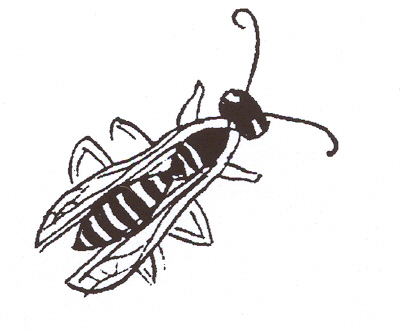
\includegraphics[angle=0,width=24mm,height=36mm]{2.jpg} 
\caption{}
\end{center}
\end{wrapfigure}



\spanenpictureLabelenpictureCaptionpictureRightentryletDatadicBody{Kitchen Cooking}
\end{center} \end{adjustwidth}  
\leftmargin 0pt{\markboth{ \headwordggoTeluINentryletDatadicBody అట్లాంటిక్ సమ్దుర్}{ \headwordggoTeluINentryletDatadicBody అట్లాంటిక్ సమ్దుర్}\headwordggoTeluINentryletDatadicBody{అట్వల్}} \spanenpronunciationggofonipaxemicpronunciationsentryletDatadicBody{[}\spanggofonipaxemicpronunciationggofonipaxemicpronunciationsentryletDatadicBody{aṭval}\spanenpronunciationggofonipaxemicpronunciationsentryletDatadicBody{]} \spanteLexSensepublishStemGlossPubLdtesensesensesentryletDatadicBody{వంట చేయుట} \spanggoTeluINexampleggoTeluINexamplessensesensesentryletDatadicBody{తిందన్ సాటి రోజి గాటోంగ్ కుస్రింగ్ అట్వల్.} \spantetranslationLdtetranslationsexamplessensesensesentryletDatadicBody{తినడానికి రోజు అన్నము కూరలు వంట చేయడం.} \end{hanglist} \end{adjustwidth} 
\begin{adjustwidth}{1pt}{0pt}{2pt}{9pt}
 \begin{hanglist}[12pt] \item 
\leftmargin 0pt{\markboth{ \headwordggoTeluINentryletDatadicBody అట్వల్}{ \headwordggoTeluINentryletDatadicBody అట్వల్}\headwordggoTeluINentryletDatadicBody{అడంతొర్}} \spanenpronunciationggofonipaxemicpronunciationsentryletDatadicBody{[}\spanggofonipaxemicpronunciationggofonipaxemicpronunciationsentryletDatadicBody{aḍantor}\spanenpronunciationggofonipaxemicpronunciationsentryletDatadicBody{]} \spanenpartofspeechengrammaticalinfosensesensesentryletDatadicBody{n} \spanendefinitionensensesensesentryletDatadicBody{crying} \spanteLexSensepublishStemGlossPubLdtesensesensesentryletDatadicBody{ఏడ్వడం} \spanggoTeluINexampleggoTeluINexamplessensesensesentryletDatadicBody{కాండిర్ పుట్త బరొబర్ అడంతెర్.} \spantetranslationLdtetranslationsexamplessensesensesentryletDatadicBody{పిల్లలు పుట్టినప్పుడు ఏడుస్తారు.} \end{hanglist} \end{adjustwidth} 
\begin{adjustwidth}{1pt}{0pt}{2pt}{9pt}
 \begin{hanglist}[12pt] \item 
\leftmargin 0pt{\markboth{ \headwordggoTeluINentryletDatadicBody అడంతొర్}{ \headwordggoTeluINentryletDatadicBody అడంతొర్}\headwordggoTeluINentryletDatadicBody{అడ్డంఅసి}} \spanenpronunciationggofonipaxemicpronunciationsentryletDatadicBody{[}\spanggofonipaxemicpronunciationggofonipaxemicpronunciationsentryletDatadicBody{aḍḍaṁasi}\spanenpronunciationggofonipaxemicpronunciationsentryletDatadicBody{]} \end{hanglist} \end{adjustwidth} 
\begin{adjustwidth}{1pt}{0pt}{2pt}{9pt}
 \begin{hanglist}[12pt] \item 
\leftmargin 0pt{\markboth{ \headwordggoTeluINentryletDatadicBody అడ్డంఅసి}{ \headwordggoTeluINentryletDatadicBody అడ్డంఅసి}\headwordggoTeluINentryletDatadicBody{అడ్డబుడ్డ}} \spanenpronunciationggofonipaxemicpronunciationsentryletDatadicBody{[}\spanggofonipaxemicpronunciationggofonipaxemicpronunciationsentryletDatadicBody{aḍḍabuḍḍa}\spanenpronunciationggofonipaxemicpronunciationsentryletDatadicBody{]} \spanenpartofspeechengrammaticalinfosensesensesentryletDatadicBody{adj} \spanendefinitionensensesensesentryletDatadicBody{blockage} \spantexitemteLexSensepublishStemGlossPubLdtesensesensesentryletDatadicBody{అడ్డదిడ్డమైన} \spanhixitemhiLexSensepublishStemGlossPubLdtesensesensesentryletDatadicBody{बाधा देने वाला} \spanggoTeluINexampleggoTeluINexamplessensesensesentryletDatadicBody{కామ్ కీయ్నెకె ఆడ బుడ్డ అయ్వ.} \spantetranslationLdtetranslationsexamplessensesensesentryletDatadicBody{పని చేసేటప్పుడు అడ్డదిడ్డముగా రావద్దు.} \end{hanglist} \end{adjustwidth} 
\begin{adjustwidth}{1pt}{0pt}{2pt}{9pt}
 \begin{hanglist}[12pt] \item 
\leftmargin 0pt{\markboth{ \headwordggoTeluINentryletDatadicBody అడ్డబుడ్డ}{ \headwordggoTeluINentryletDatadicBody అడ్డబుడ్డ}\headwordggoTeluINentryletDatadicBody{అడ్డమ్}} \spanenpronunciationggofonipaxemicpronunciationsentryletDatadicBody{[}\spanggofonipaxemicpronunciationggofonipaxemicpronunciationsentryletDatadicBody{aḍḍam}\spanenpronunciationggofonipaxemicpronunciationsentryletDatadicBody{]} \spanenpartofspeechengrammaticalinfosensesensesentryletDatadicBody{adv} \spanendefinitionensensesensesentryletDatadicBody{across.} \spantexitemteLexSensepublishStemGlossPubLdtesensesensesentryletDatadicBody{అడ్డముగా} \spanhixitemhiLexSensepublishStemGlossPubLdtesensesensesentryletDatadicBody{आडा} \spanggoTeluINexampleggoTeluINexamplessensesensesentryletDatadicBody{పోడ్దున్ అడ్డమ్ టెప్ప ఆత.} \spantetranslationLdtetranslationsexamplessensesensesentryletDatadicBody{సూర్యునికి అడ్డముగా మేఘం వచ్చింది.} \end{hanglist} \end{adjustwidth} 
\begin{adjustwidth}{1pt}{0pt}{2pt}{9pt}
 \begin{hanglist}[12pt] \item 
\leftmargin 0pt{\markboth{ \headwordggoTeluINentryletDatadicBody అడ్డమ్}{ \headwordggoTeluINentryletDatadicBody అడ్డమ్}\headwordggoTeluINentryletDatadicBody{అడ్డమ్ ఆ}} \spanenpronunciationggofonipaxemicpronunciationsentryletDatadicBody{[}\spanggofonipaxemicpronunciationggofonipaxemicpronunciationsentryletDatadicBody{aḍḍam ā-}\spanenpronunciationggofonipaxemicpronunciationsentryletDatadicBody{]} \spanenpartofspeechengrammaticalinfoentryletDatadicBody{v} \xsensenumbersensesensesentryletDatadicBody{1}\xsensenumberaftersensesensesentryletDatadicBody{) }\spanendefinitionensensesensesentryletDatadicBody{object} \spantexitemteLexSensepublishStemGlossPubLdtesensesensesentryletDatadicBody{అడ్డుకో} \spanhixitemhiLexSensepublishStemGlossPubLdtesensesensesentryletDatadicBody{रोक; बीच में पड} \spanggoTeluINexampleggoTeluINexamplessensesensesentryletDatadicBody{బాబల్ బయ్యెన్ పానెకె కాండి అడ్డమ్ ఆతొర్.} \spantetranslationLdtetranslationsexamplessensesensesentryletDatadicBody{నాన అమ్మను కొట్టే టప్పుడు కొడుకు అడ్డుకున్నాడు.} \xsensenumbersensesensesentryletDatadicBody{2}\xsensenumberaftersensesensesentryletDatadicBody{) }\spanendefinitionensensesensesentryletDatadicBody{obstruct} \spantexitemteLexSensepublishStemGlossPubLdtesensesensesentryletDatadicBody{అడ్డగించు} \spanhixitemhiLexSensepublishStemGlossPubLdtesensesensesentryletDatadicBody{रोक; मना कर} \spanggoTeluINexampleggoTeluINexamplessensesensesentryletDatadicBody{నిమ్మె దర్బర్‌తె అడ్డమ్ అస్సి వడ్క్‌మా.} \spantetranslationLdtetranslationsexamplessensesensesentryletDatadicBody{నువ్వు కూర్చోవడం కన్నా అడ్డంగా మాట్లాడకు.} \end{hanglist} \end{adjustwidth} 
\begin{adjustwidth}{1pt}{0pt}{2pt}{9pt}
 \begin{hanglist}[12pt] \item 
\leftmargin 0pt{\markboth{ \headwordggoTeluINentryletDatadicBody అడ్డమ్ ఆ}{ \headwordggoTeluINentryletDatadicBody అడ్డమ్ ఆ}\headwordggoTeluINentryletDatadicBody{అడ్డంవడి}} \spanenpronunciationggofonipaxemicpronunciationsentryletDatadicBody{[}\spanggofonipaxemicpronunciationggofonipaxemicpronunciationsentryletDatadicBody{aḍḍanvaḍi}\spanenpronunciationggofonipaxemicpronunciationsentryletDatadicBody{]} \spanendefinitionensensesensesentryletDatadicBody{air coming across} \spanteLexSensepublishStemGlossPubLdtesensesensesentryletDatadicBody{అడ్డంగా వచ్చే గాలి} \spanggoTeluINexampleggoTeluINexamplessensesensesentryletDatadicBody{నిన్నెతల్ అడ్డంవడి వాసెర్ మంత.} \spantetranslationLdtetranslationsexamplessensesensesentryletDatadicBody{నిన్నటి నుండి అడ్డంగా గాలి వస్తుంది.} \end{hanglist} \end{adjustwidth} 
 \end{multicols}\begin{center}
\topskip 18pt{\baselineskip 18pt{\letterletHeaddicBody{న}}}\end{center} 
 \setlength{\columnsep}{12pt} 
\setlength\columnseprule{0.4pt} 
\begin{multicols}{2}{\raggedright} \begin{adjustwidth}{1pt}{0pt}{2pt}{9pt}
 \begin{hanglist}[12pt] \item 
\leftmargin 0pt{\markboth{ \headwordggoTeluINentryletDatadicBody అడ్డంవడి}{ \headwordggoTeluINentryletDatadicBody అడ్డంవడి}\headwordggoTeluINentryletDatadicBody{-న్గ}} \spanenpronunciationggofonipaxemicpronunciationsentryletDatadicBody{[}\spanggofonipaxemicpronunciationggofonipaxemicpronunciationsentryletDatadicBody{nga}\spanenpronunciationggofonipaxemicpronunciationsentryletDatadicBody{]} \end{hanglist} \end{adjustwidth} 
\begin{adjustwidth}{1pt}{0pt}{2pt}{9pt}
 \begin{hanglist}[12pt] \item 
\leftmargin 0pt{\markboth{ \headwordggoTeluINentryletDatadicBody -న్గ}{ \headwordggoTeluINentryletDatadicBody -న్గ}\headwordggoTeluINentryletDatadicBody{-న్గటల్}} \spanenpronunciationggofonipaxemicpronunciationsentryletDatadicBody{[}\spanggofonipaxemicpronunciationggofonipaxemicpronunciationsentryletDatadicBody{ngaṭal}\spanenpronunciationggofonipaxemicpronunciationsentryletDatadicBody{]} \end{hanglist} \end{adjustwidth} 
 \end{multicols}\begin{center}
\topskip 18pt{\baselineskip 18pt{\letterletHeaddicBody{ు}}}\end{center}
 \setlength{\columnsep}{12pt} 
\setlength\columnseprule{0.4pt} 
\begin{multicols}{2}{\raggedright} \begin{adjustwidth}{1pt}{0pt}{2pt}{9pt}
 \begin{hanglist}[12pt] \item 
\leftmargin 0pt{\markboth{ \headwordggoTeluINentryletDatadicBody -న్గటల్}{ \headwordggoTeluINentryletDatadicBody -న్గటల్}\headwordggoTeluINentryletDatadicBody{-ున్‌}} \spanenpronunciationggofonipaxemicpronunciationsentryletDatadicBody{[}\spanggofonipaxemicpronunciationggofonipaxemicpronunciationsentryletDatadicBody{un‌}\spanenpronunciationggofonipaxemicpronunciationsentryletDatadicBody{]} \spanenpartofspeechengrammaticalinfosensesensesentryletDatadicBody{ns} \spanendefinitionensensesensesentryletDatadicBody{ACC} \end{hanglist} \end{adjustwidth} 
\begin{adjustwidth}{1pt}{0pt}{2pt}{9pt}
 \begin{hanglist}[12pt] \item 
\leftmargin 0pt{\markboth{ \headwordggoTeluINentryletDatadicBody -ున్‌}{ \headwordggoTeluINentryletDatadicBody -ున్‌}\headwordggoTeluINentryletDatadicBody{-ుర్}} \spanenpronunciationggofonipaxemicpronunciationsentryletDatadicBody{[}\spanggofonipaxemicpronunciationggofonipaxemicpronunciationsentryletDatadicBody{ur}\spanenpronunciationggofonipaxemicpronunciationsentryletDatadicBody{]} \spanenpartofspeechengrammaticalinfosensesensesentryletDatadicBody{vs} \spanendefinitionensensesensesentryletDatadicBody{3.M.PL.DIST} \end{hanglist} \end{adjustwidth} 
 \end{multicols}\begin{center}
\topskip 18pt{\baselineskip 18pt{\letterletHeaddicBody{ొ}}}
 \label{last_pageొ} 
\end{center}
 \setlength{\columnsep}{12pt} 
\setlength\columnseprule{0.4pt} 
\begin{multicols}{2}{\raggedright} \begin{adjustwidth}{1pt}{0pt}{2pt}{9pt}
 \begin{hanglist}[12pt] \item 
\leftmargin 0pt{\markboth{ \headwordggoTeluINentryletDatadicBody -ుర్}{ \headwordggoTeluINentryletDatadicBody -ుర్}\headwordggoTeluINentryletDatadicBody{-ొర్}} \spanenpronunciationggofonipaxemicpronunciationsentryletDatadicBody{[}\spanggofonipaxemicpronunciationggofonipaxemicpronunciationsentryletDatadicBody{or}\spanenpronunciationggofonipaxemicpronunciationsentryletDatadicBody{]} \spanenpartofspeechengrammaticalinfosensesensesentryletDatadicBody{vs} \spanendefinitionensensesensesentryletDatadicBody{3.M.SG} \end{hanglist} \end{adjustwidth} 
 \end{multicols}
\end{document}
